\subsection{A linear storage cascade instead of Richards' equation (LAG)}\label{sec:szvadoselag}
Where only the delay and spreading of recharge through the unsaturated zone matter, \cmd{:SoilZoneVadose LAG} replaces
Richards' equation by a linear storage cascade on the same column: the same nodes, contents, equilibrium profile,
water-table following and hotstart (\cmd{:GWVadoseColumns}) as \cmd{RICHARDS} (Section~\ref{sec:szvadose}); only the
step differs. The water node $i$ holds above its equilibrium content,
\begin{equation}
S_i=(\theta_i-\theta_{\mathrm{eq},i})\,\Delta z_i,\qquad \frac{dS_i}{dt}=Q_{i-1}-Q_i,\qquad Q_i=\frac{\max(S_i,0)}{k_i},\qquad k_i=t_m\,\Delta z_i,
\end{equation}
is the store of a linear reservoir with residence time $k_i$; $Q_0=q_{\mathrm{top}}$ is the column's inflow and $Q_N$ the
flux into the water table, which replaces the column's share of the recharge in \cmd{RCH\_RAVEN}. $t_m$ [d/m] is the travel
time per metre of the node's material, so the mean travel time through a column of one material is $\sum_ik_i=t_mL$ (a
linear kinematic wave of celerity $1/t_m$, discretized as a cascade). Each node uses its own material's $t_m$, so a
column crossing sloping layers of different aquifer classes is a cascade of different residence times.

\paragraph{Travel time.} \cmd{:SoilZoneVadose LAG} $t_m$ gives $t_m$ for every material. Without it (or with 0) $t_m$
is derived per material from the celerity of a kinematic wave at a reference flux $q_r=1$~mm/d, with the conductivity
$K=K_sS_e^{\varepsilon}$, $S_e=(\theta-\theta_s+S_y)/S_y$, $\varepsilon=2b+3$ (Campbell's exponent):
$c=dK/d\theta=\varepsilon q/(S_yS_{e,r})$ at $K=q$, and
\begin{equation}\label{eq:lagtm}
t_m=\frac1c=\frac{S_y\,S_{e,r}}{\varepsilon\,q},\qquad S_{e,r}=\Big(\frac{q}{K_s}\Big)^{1/\varepsilon},\qquad q=\min(q_r,K_s).
\end{equation}
A material with $K_s<q_r$ cannot carry the reference flux: then $q=K_s$, $S_{e,r}=1$ and $t_m=S_y/(\varepsilon K_s)$. $K_s$ =
\cmd{K\_VERT}, $S_y$ = \cmd{SPEC\_YIELD}, $b$ = \cmd{CLAPP\_B} of the aquifer class (for an existing model: the model's
\cmd{K33}/\cmd{K} and \cmd{SY}, and \cmd{CLAPP\_B} of \cmd{:SoilZoneAquiferClass}). The derived value is a starting point;
the travel time is the method's one calibration parameter.

\begin{example}[: derived travel times]
Sand ($K_s=5$~m/d, $S_y=0.25$, $b=4$, $\varepsilon=11$): $S_{e,r}=(0.001/5)^{1/11}=0.461$, $t_m=0.25\times0.461/(11\times0.001)=10.5$~d/m.
Loam ($K_s=0.25$~m/d, $S_y=0.15$, $b=5.4$, $\varepsilon=13.8$): $S_{e,r}=0.670$, $t_m=7.3$~d/m.
Clay ($K_s=2\times10^{-4}$~m/d $<q_r$, $S_y=0.05$, $b=11$, $\varepsilon=25$): $t_m=0.05/(25\times2\times10^{-4})=10.0$~d/m.
A 5~m unsaturated zone in the sand delays recharge by about 52 days on average. The three are similar because a
large $S_y$ (much water to move) offsets a large $K_s$ at the same small flux; at a larger flux the wave is faster
(here the derivation fixes $q_r$). These values are unit test U of \cmd{test\_vz\_lag.py}.
\end{example}

\paragraph{Spreading.} The spread of the response is set by the node count: its variance is $\sum_ik_i^2$, so the
cascade spreads like $N_{\mathrm{eff}}=(\sum_i k_i)^2/\sum_i k_i^2$ equal reservoirs (for equal ones the response is the
Erlang (gamma) density), with a relative spread $1/\sqrt{N_{\mathrm{eff}}}$. The grid is that of the Richards column (thin
nodes at both ends, growing by 1.3 towards the middle up to $1.3^8$ times the end nodes, $\lceil L/0.05\text{ m}\rceil$
nodes but at least 3 and at most $N$), so $N_{\mathrm{eff}}<N$; beyond 18 nodes the extra ones are of equal thickness and
$N_{\mathrm{eff}}$ grows as about $N-7$. For a column of one material
\begin{center}\small
\begin{tabular}{lcccccccccc}\toprule\hdr
nodes $N$ & 3 & 4 & 6 & 8 & 12 & 16 & 24 & 32 & 50 & 100\\\midrule
$N_{\mathrm{eff}}$ & 2.95 & 3.93 & 5.74 & 7.38 & 10.1 & 12.0 & 17.7 & 25.3 & 43.1 & 93.0\\\bottomrule
\end{tabular}\end{center}
The node count therefore sets the spreading, from a broad response ($N=3$, spread 58\% of the mean) through 29\% for
the default 16 nodes to 15\% for 50 and 10\% for 100; columns shorter than $N\times5$~cm have fewer nodes (at least 3)
(Figure~\ref{fig:vzlagcascade}, left).

\paragraph{The step.} Each Raven step is divided into $n$ equal substeps no longer than the shortest residence time,
$n=\min\big(\max(\lceil\dt/\min_ik_i\rceil,1),50\big)$ (computed in floating point and clamped before it is made an
integer: a tiny residence time, with 200 nodes or \cmd{LAG 1e-6}, would overflow an integer). In
each substep every node, top down, is solved exactly with the constant inflow its upper neighbour released in that
substep,
\begin{equation}
S_i(t+h)=S_i(t)\,e^{-h/k_i}+I_ik_i\big(1-e^{-h/k_i}\big),\qquad \text{outflow } S_i(t)+I_ih-S_i(t+h),
\end{equation}
so the nodes pass on exactly what they release and the column conserves water to round-off; $q_{\mathrm{bot}}$ is taken
from the storage change as for \cmd{RICHARDS}. The piecewise-constant transfer between nodes is the only approximation:
against the exact cascade the cumulative response of the default 16-node column differs by at most 1.1\% of the
impulse with daily steps, and the mean travel time by 0.4\%.
A node may not hold more than its porosity, $S_i\le S_{\max,i}=(\theta_s-\theta_{\mathrm{eq},i})\Delta z_i$: water beyond
it passes on to the next node within the substep, and from the last node into the water table. In the capillary
fringe, where $\theta_{\mathrm{eq}}$ is close to $\theta_s$, nodes have almost no room and water crosses it at once; a
large inflow fills the top nodes to saturation and advances as a front at $q/(\theta_s-\theta_{\mathrm{eq}})$, the speed
of a sharp front. A column therefore takes any inflow: nothing is rejected at its top (the soil zone's percolation and
the saturated fraction limit what reaches it); an upward demand ($q_{\mathrm{top}}<0$) is rejected entirely, since
capillary rise into the soil zone comes from the water table through the column by the steady formula
(Section~\ref{sec:szcaprise}), even where a column is active; and an inactive column rejects its inflow and returns
nothing (the contract shared by all methods). A node below equilibrium ($S_i<0$) does not drain; inflow first fills
it. That state arises only from a hotstart written by another method (\cmd{:GWVadoseColumns} of a \cmd{RICHARDS} run:
contents below equilibrium after evaporation or capillary rise): a moving water table remaps the excess and the
equilibrium together, and the cascade itself never takes a node below equilibrium.

\paragraph{Steady start.} With \cmd{:SoilZoneVadoseInitialFlux} $q$ the cascade starts at its steady state,
$S_i=\min(q\,k_i,\,S_{\max,i})$ (a full node passes everything it receives), which delivers $q$ from the first step (unit
test U: to round-off).

\paragraph{Behaviour to expect.} With three depth classes (\cmd{:SoilZoneVadoseClasses 3}) the water table can be lower
during rain than with one class: the upper classes' columns are long (5 to 13~m in the rough-terrain case R20) and hold
more of the rain in transit. That is the method's own physics, not an error. The cascade has no conductivity limit: a
full column passes any inflow, however slowly permeable its material; where the permeability limits recharge, use
\cmd{RICHARDS} or \cmd{KINEMATIC}.

\begin{example}[: the storm of P1 with LAG]
A 3-day storm of 40~mm/d over a water table 6~m deep, sand with $K_s=0.5$ m/d, $S_y=0.2$, $b=4$ (test L1 of
\cmd{test\_vz\_lag.py}; the case of P1). Without a column the recharge's centroid is on day~6.1; with \cmd{RICHARDS} on
day~15.6. The soil's percolation of the first days (50~mm/d) and the storm pass the capillary fringe (0.3~m) at once and the
storm fills the top nodes. With \cmd{LAG 2} the centroid is on day~13.9 and the peak 30\% below the no-column run, with
\cmd{LAG 4} on day~21.1, and with the derived travel time ($t_m=10.3$~d/m) on day~40.9: delays of 8 to 35 days set by
$t_m$ (Figure~\ref{fig:vzlagcascade}, right). Every identity holds to round-off (largest $4\times10^{-10}$).
\end{example}

\begin{figure}[!htbp]\centering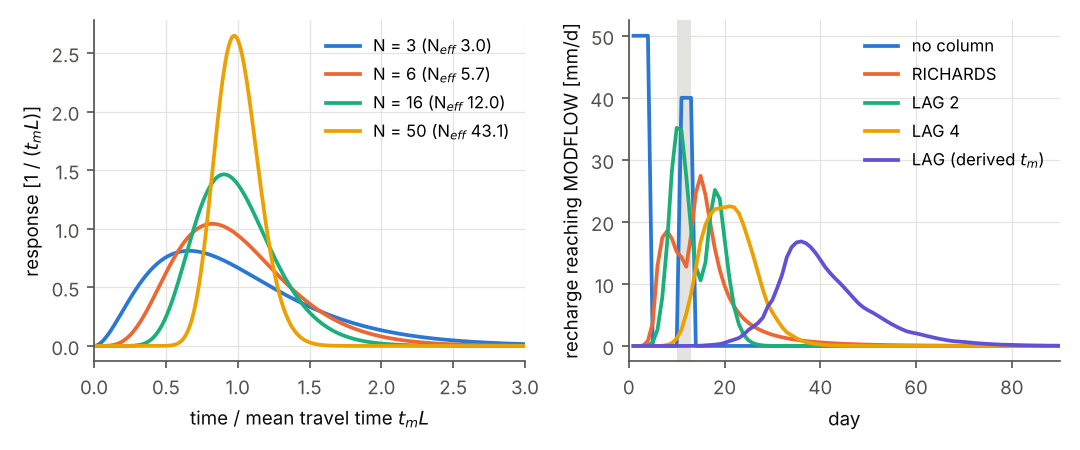
\includegraphics[width=\linewidth]{figures/fig_vz_lag_cascade.png}
\caption{Left: response of a column of one material to an impulse of water at its top, for 3 to 50 nodes on the
column grid (exact cascade; time in units of the mean travel time $t_mL$). Right: recharge reaching MODFLOW in test L1
(3-day storm, grey, over a 6~m unsaturated zone, after four days of percolation from the initial soil water): without a
column, with \cmd{RICHARDS}, and with \cmd{LAG} 2, 4 and the derived travel time.}\label{fig:vzlagcascade}
\end{figure}

\paragraph{Cost and limits.} A column step costs 1 to 3~$\mu$s for 16 nodes (unit test U: 1.7 to 2~$\mu$s), against
12 to 15~$\mu$s for \cmd{RICHARDS}; in a coupled run the water-table following, which remaps the nodes every step (as for
\cmd{RICHARDS}), and the interface iteration cost as much again (test S: 400 columns over a year add 1.4~s to a 1.7~s
run, \cmd{RICHARDS} 2.3~s). The spreading narrows only as $1/\sqrt{N-7}$ with more nodes (each costs time). The cascade
knows no suction: it neither holds water against gravity nor lets the column dry, and its delay does not depend on the
flux (only on $t_m$): a wet year travels as fast as a dry one.

\begin{refcard}{LAG unsaturated columns}
\textbf{Sources/sinks.} Between the soil-zone base and the water table of every exchange column: inflow the column's
unsaturated share of the recharge, outflow to MODFLOW's recharge (\cmd{RCH\_RAVEN}).\par\smallskip
\textbf{Constraints/notes.} Linear reservoirs $k_i=t_m\Delta z_i$ on the Richards grid and its equilibrium profile; mass
conserved to round-off; no content above $\theta_s$; nothing rejected at the top of an active column; capillary rise from
the water table (steady formula); saved in \cmd{solution.rvc} (\cmd{:GWVadoseColumns}), interchangeable with the other
methods' hotstarts.\par\smallskip
\par\noindent\begin{minipage}{\linewidth}\textbf{Command syntax}
\begin{lstlisting}
# .rvg
:SoilZoneVadose LAG          # derived travel time per material (q_r = 1 mm/d), 16 nodes at most
:SoilZoneVadose LAG 4 8      # t_m = 4 d/m for every material, 8 nodes at most (3 to 200)
:SoilZoneVadose LAG 0 24     # derived travel time, 24 nodes (N_eff about 18)
\end{lstlisting}
\end{minipage}\par\smallskip
\par\noindent\begin{minipage}{\linewidth}\textbf{Parameters}\par\smallskip
\begin{tabular}{>{\raggedright\arraybackslash}P{0.09\linewidth}>{\raggedright\arraybackslash}P{0.26\linewidth}>{\raggedright\arraybackslash}P{0.283\linewidth}>{\raggedright\arraybackslash}P{0.1\linewidth}>{\raggedright\arraybackslash}P{0.15\linewidth}}\toprule\hdr Symbol & Parameter & Class (where it is set) & Units & Reference\\\midrule
$t_m$ & travel time per metre & \cmd{:SoilZoneVadose LAG} (0: Eq.~\eqref{eq:lagtm}) & d/m & Sec.~\ref{sec:szvadoselag}\\
$N$ & nodes at most & \cmd{:SoilZoneVadose LAG} & -- & Sec.~\ref{sec:szvadose}\\
$K_s$, $S_y$, $b$ & \cmd{K\_VERT}, \cmd{SPEC\_YIELD}, \cmd{CLAPP\_B} & aquifer class (\cmd{:AquiferClasses}) & m/d, --, -- & Sec.~\ref{app:class}\\
$\theta_s$, $\psi_a$ & \cmd{POROSITY}, \cmd{AIR\_ENTRY\_PRESSURE} & aquifer class (equilibrium profile, room) & --, m & Sec.~\ref{app:class}\\
\bottomrule\end{tabular}\end{minipage}\par\smallskip
\textbf{Outputs.} \cmd{GWBudget.csv}: \emph{unsaturated zone inflow}, \emph{unsaturated zone to aquifer},
\emph{unsaturated zone storage} (capillary rise to the soil zone 0: the rise comes from the water table);
\cmd{GWModelSummary.txt}: the method and its nodes.
\end{refcard}

\paragraph{Verification.} \cmd{test\_vz\_lag.py}: U (unit tests: travel times, mass balance to $5\times10^{-16}$ of the
flows and storage over 16\,000 random steps of 400 random columns, no content above $\theta_s$, nodes below
equilibrium, inactive columns, tiny residence times, steady start, Erlang response of equal reservoirs within 0.6\%,
impulse responses of grid columns against the exact cascade within 1.1\%), L1 (above), L2 (a water table rising
through the columns into the soil zone and falling again), L3 (a column across two aquifer classes on a slope), L4
(restart 60 + 60 days against 120 days: $2\times10^{-8}$), L5 (existing-model round trip: $2.4\times10^{-4}$), S (cost) and B
(\cmd{NONE}, \cmd{RICHARDS} and \cmd{CONCEPTUAL} runs byte-identical to a build without \cmd{LAG}).
